\chapter{2020-05-12-Discuss ITransE}

\section{Model Architecture}
There are two assumptions in our idea: 
\begin{enumerate}
    \item The cross-graph neighbours representation augmentation is helpful.
    \item Aligned entities can supervise the training.
\end{enumerate}
In this week, I am focusing on the first assumption. The model architecture can be seen from Figure \ref{fig:model_architecture_2020_0512}. 
\begin{figure}[!ht]
    \centering
    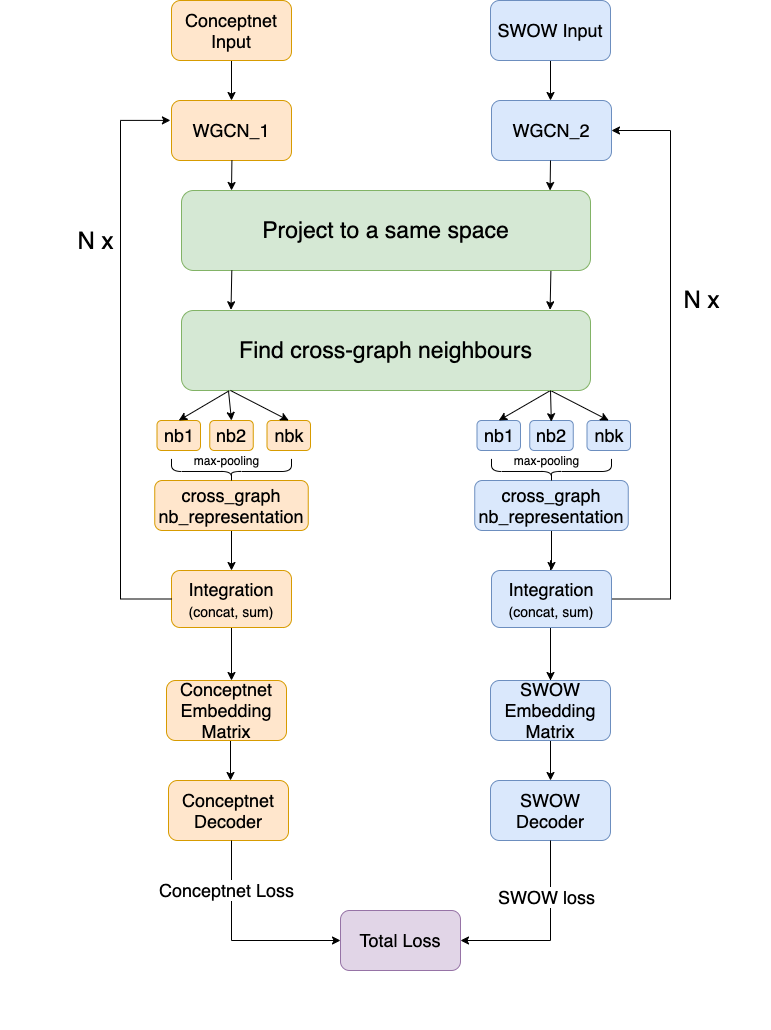
\includegraphics[scale=0.4]{images/0512/model-architecture-2020-05-12.png}
    \caption{Model Architecture}
    \label{fig:model_architecture_2020_0512}
\end{figure}

\section{Experimental Results}
The experimental results are shown in Figure\ref{fig:experimental_results}. 
\begin{figure}
    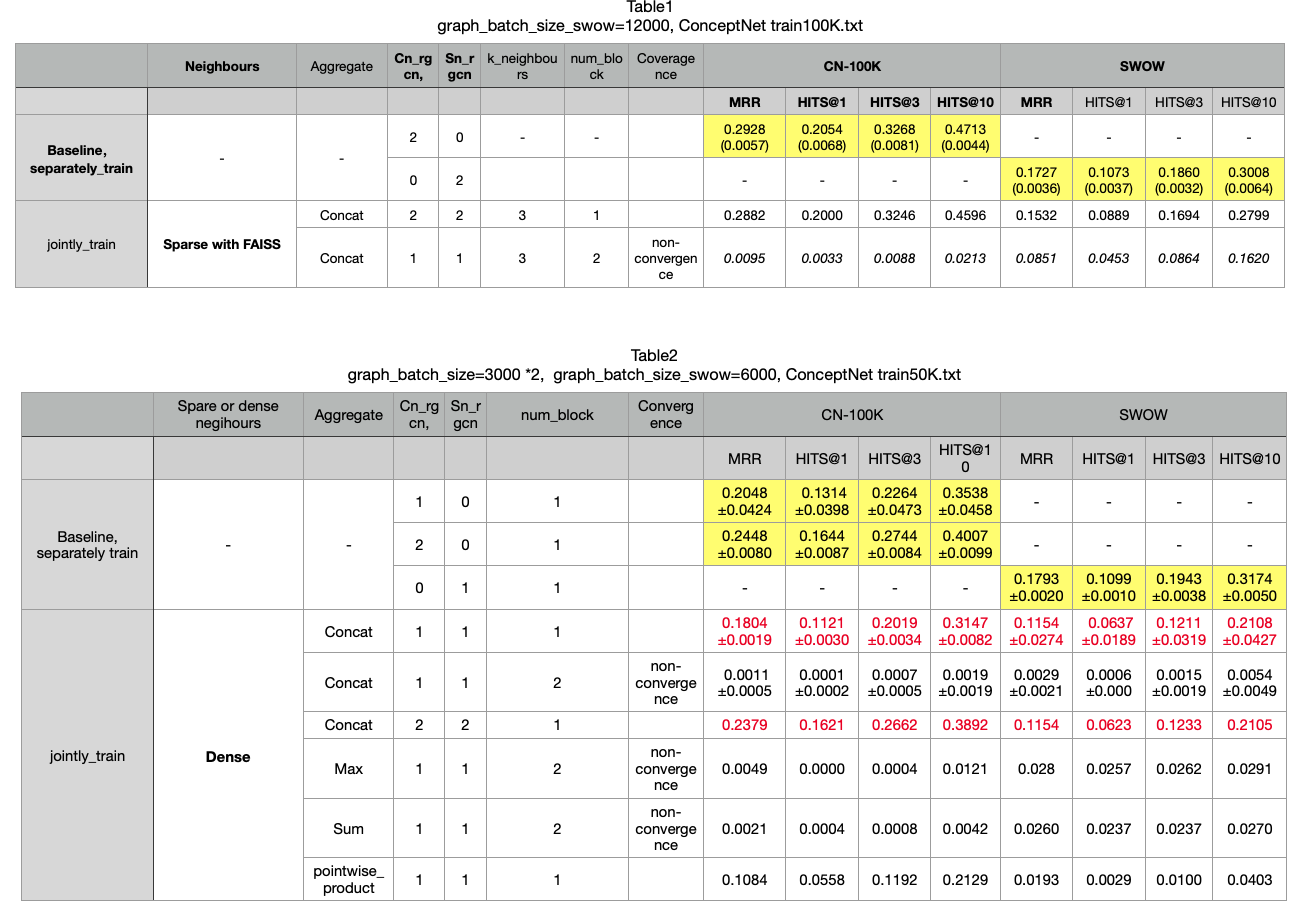
\includegraphics[scale=0.36]{images/0512/results-2020-05-12.png}
    \caption{Experimental Results}
    \label{fig:experimental_results}
\end{figure}

Table1 is the results of using FAISS to retrieve the topk nearest neighbours and get a vector representation for them with max-pooling. 
Table2 is replace the neighbour representation with the attention weight from $A=E_c E_s^T$. The ConceptNet training set in Table2 is decreased from 100K to 50K, because of the memory is not enough for the two big embedding matrix to multiply. Also, the graph\_batch\_size is decrease from 12,000 to 6,000. So the numbers will be different.

When block\_num is 1, I was trying to test whether the cross-graph neighbours representation can introduce extra knowledge and increase the performance. Compared with the baseline results, which is separately trained in each graph, the results of jointly training dropped. 

When block\_num is set to 2, I was trying to see whether stack the block multiple times can help the cross-graph neighbours be fused better. However, in both scenario, the model cannot converge. My guess is 1) it's too hard for the RGCN to aggregate both neighbours from its own graphs and another graph. 2) The cross-graph contains too much noise. 

So, for now, the experimental results are negative. 
\newpage
\section{Cross-graph Attention Related Work}

\cite{cao-etal-2019-multi} generate the cross-graph attention matrix to replace the adjacency matrix of GNN. The attention weight is for selecting neighbours in its own graph instead of the another graph. Their goal is to make the two sub-graphs from two different knowledge graph to share more common edges. 
\begin{align}
    \alpha_{i j}=\max _{r \in R, r^{\prime} \in R^{\prime}} \mathbf{1}\left(\left(e_{i}, r, e_{j}\right) \in T\right) \operatorname{sim}\left(r, r^{\prime}\right)
\end{align}
The attention matrix requires to compute the similarity between relation types of two graphs. However, it's not suitable for our research, because relation types in ConceptNet and SWOW are completely different. 

\cite{xu-etal-2019-cross-lingual} computes the attention matrix for each node in $G_{1}$ over all the nodes in $G_{2}$ and then combine them with the original nodes representation using a  multi-perspective cosine matching function $f_m$ before feeding them to a GCN. 
\begin{align}
    \alpha_{i, j}=\operatorname{cosine}\left(\boldsymbol{e}_{i}^{1}, \boldsymbol{e}_{j}^{2}\right) \quad j \in\left\{1, \ldots,\left|G_{2}\right|\right\} \\
    \boldsymbol{m}_{i}^{a t t}=f_{m}\left(\boldsymbol{e}_{i}^{1}, \overline{\boldsymbol{e}}_{i}^{1}\right)
\end{align}
Their matching function $f_m$ is very complicated, so I only used the dense attention idea in this week's work. 

\section{Meeting Notes}

\textbf{High level view}: 
\begin{enumerate}
    \item Can we learn the alignments?
    \item Can we use aligned seeds to help learn better nodes representation?
    \item Can better alignments help us complete the knowledge graph? 
\end{enumerate}


\noindent \textbf{To do List}: 
\begin{enumerate}
    \item  Modify current model architecture, 
        \begin{itemize}
            \item insert another gcn to integrate the integrated representation.
            \item integrate the self-graph representation and cross-graph nb representation using gate mechanism. 
        \end{itemize}
        
    \item List the difference of settings between our scenario and the ITransE \citep{Zhu2017IterativeEA}. 
    \item Try to see whether ITransE can apply to the alignments of ConceptNet and SWOW 
    \\(See does other people use their method in other bigger and sparser graph.)
\end{enumerate}





\begin{comment}
\section{ToDo}
\begin{todolist}
    \item model architecture modification\\
        remove the second layer of gcn and add the aggregation representation of cross-nb with original graph representation
       \begin{enumerate}
       \item Encode input graph with a WGCN
       \item Retrieve cross-graph neighbours 
       \item Construct cross-graph neighbours representation 
       \item Integrate self-graph representation with cross-graph representation, eg: f(W[a,b])
       \item Feed the integrated representation to WGCN (share parameters with the encoder WGCN or not share)  and repeat 1 to N times 
      \end{enumerate}       
    \item add alignment loss for supervision
        \begin{todolist}
            \item find a reasonable way to do negative sampling
        \end{todolist}
\end{todolist}

\begin{table}[]
    \centering
    \begin{tabular}{c|c}
         b&\\
         & 
    \end{tabular}
    \caption{Experiment re}
    \label{tab:my_label}
\end{table}
baseline:
 1. jointly train ConceptNet and SWOW by simply adding their loss together. 
 
 our model: 

why would I want to retrieve the cross-graph neighbours? 
\begin{itemize}
    \item In general, we want to  a bidirectional knowledge transfer between ConceptNet and SWOW. 	
\item One way could be 1. encode two graphs separately 2. Align entities in two graphs. 3. Update the representation for aligned words with representations from two graphs. We have proved that this idea can bring slight improvements for both graphs. However, we also found the limitation of this idea is that the aligned entities are limited \ref{tab:overlap-conceptnet-swow}, which means only a limited number of nodes representation will be updated. 

If we want to update more nodes, we need to increase their intersection parts.  

allow more nodes in one graph to influence the update of node representation. (What is the potential problems behind this?) 


\item  align the words in two graphs and 
\item  The aligned pair seeds in ConceptNet and SWOW are limited. If we only use the 
\end{itemize}

 each other's nearest neighbours and construct a cross-network node representation together with original graph represen
 How to speed up the process of idea verification ?
 \begin{itemize}
     \item  Hyper parameter
      \begin{itemize}
         \item reduce graph\_batch\_size 
         \item reduce training\_epochs 
         \item increase learning\_rate
    \end{itemize}
     \item data
         \begin{todolist}
         \item[\xmark] 16-bit precision , apex (ony support V100, TiTAN V)
         \item data Loader?  \href{https://towardsdatascience.com/9-tips-for-training-lightning-fast-neural-networks-in-pytorch-8e63a502f565}{here}
           \end{todolist}
     \item code 
       
 \end{itemize}

I am thinking the improvements of \cite{Malaviya2019ExploitingSA} comes a lot from the BERT model. Nodes in valid and test are fine-tuned on BERT model, even though they cannot be trained through GCN.
\section{Papers: deep graph matching}
do they compute similarity between all the nodes of two graphs or only select top-k nearest neighbours 
how do they integrate the attentive-representation and the original representation? 
%看是否有人 用sparsemax 选择neighbours
Do they have negative sampling? How do they do? 
Recently, graph neura
networks have become a focus of research leading to various proposed deep graph matching techniques (Wang et al., 2019b; Zhang & Lee, 2019; Xu et al., 2019d; Derr et al., 2019). 
Wang et al. (2019b) use node-wise features in
combination with dense node-to-node cross-graph affinities, distribute them in a local fashion, and
adopt sinkhorn normalization for the final task of linear assignment


\begin{align}
    \mathbf{m}_{j \rightarrow i}=f_{\text {message }}\left(\mathbf{h}_{i}^{(t)}, \mathbf{h}_{j}^{(t)}, \mathbf{e}_{i j}\right), \forall(i, j) \in E_{1} \cup E_{2} \\
    \boldsymbol{\mu}_{j \rightarrow i}=& f_{\text {match }}\left(\mathbf{h}_{i}^{(t)}, \mathbf{h}_{j}^{(t)}\right)   \forall i \in V_{1}, j \in V_{2}, \text { or } i \in V_{2}, j \in V_{1} \\
    \mathbf{h}_{i}^{(t+1)}=f_{\mathrm{node}}\left(\mathbf{h}_{i}^{(t)}, \sum_{j} \mathbf{m}_{j \rightarrow i}, \sum_{j^{\prime}} \boldsymbol{\mu}_{j^{\prime} \rightarrow i}\right)

\end{align}
\end{comment}